\documentclass{sig-alternate}
\usepackage[ruled]{algorithm2e}
\usepackage{url}
\usepackage{graphicx}
\usepackage{paralist}
\usepackage{times}
\usepackage{latexsym}
\usepackage{amsmath,amssymb}
\usepackage{url}
\usepackage{color}
\usepackage{graphicx}
\usepackage{algpseudocode}
\usepackage{epstopdf}
\usepackage{dsfont,pifont}
\usepackage{bbm}
\usepackage{booktabs}
\usepackage[english]{babel}
\usepackage{framed}
\usepackage{multicol,multirow}
\usepackage{CJK}
\usepackage{indentfirst}
\usepackage{amsmath}
\usepackage{listings}
\usepackage{caption}
\usepackage{subcaption}
\newcommand{\subparagraph}{}
\usepackage{float}
\usepackage{multirow}
\usepackage{tabularx}
\graphicspath{{./figures/}}


\begin{document}
\title{Design and Implementation of a RISC Simulator}
\numberofauthors{2} 
\author{
\alignauthor {Wei Hong \\\email{weihong@cs.umass.edu}} 
\alignauthor {Tengyu Sun \\\email{tsun@cs.umass.edu}} 
\and
\affaddr{College of Computer Science, University of Massachusetts} \\ \affaddr{Amherst, MA 01003} \\
}

\date{\today}
\maketitle
\abstract
In this report, we designed a MIPS-like instruction set and implemented a simulator for it. The simulator supports cached memory and pipelined instruction execution. In order to evaluate its performance, we designed several benchmarks and compared the clock cycles under various simulator configurations.

\section{Introduction}
This report describes the design and implementation of a RISC instruction set and its simulator. The instruction set is a subset of the MIPS instruction set\footnote{\url{https://imgtec.com/mips/architectures/mips64/}} with some modifications for simplicity. It supports basic instructions such as data transfer, control, integer and floating point computations as well as the advanced feature SIMD. The simulator is implemented in C++ with QT for the GUI. The backbone consists of a hierarchical multi-way associative memory cache system and a pipelined CPU architecture with a Floating Point Unit (FPU) and a Vector Unit (VU). A few benchmarks including exchange sort and matrix multiplication are used to evaluate the performance of the simulator.

The report is structured as follows: in section 2, we will introduce the design of our instruction set and in section 3, we will describe the implementation of the simulator. Then in section 4, we will report the performance evaluation results.  At last, we will summarize the lessons learned in section 5.

\section{Instruction Set Design}
The instruction set follows the RISC design strategy. It contains 6 types of instructions, i.e., data transfer, arithmetic and logical, control, floating point, cache and SIMD. The data types supported are 8-bit byte, 32-bit word integer and 32-bit single precision floating point. The memory is byte addressable and the byte ordering is big-endian. Word access requires 4-byte alignment. 

There are 16 32-bit general purpose registers for integers (gpr[0] - gpr[15]), 16 32-bit registers for floating point (fpr[0] - fpr[15]), and 16 64-bit vector registers for SIMD (vr[0] - v[15]). General purpose and floating point registers can be accessed by load/store instructions. gpr[15] is usually used by control instructions as the default register for storing return address. Vector registers can hold 8 8-bit byte integers simultaneously. The vector element index starts from the most significant bit, that is vr[i][0] is the higher 8 bits of vr[i]. There are also one 32-bit register for program counter (\$pc) and one 32-bit status register (\$status). \$pc cannot be directly accessed and can only be changed by control instructions.

Instructions use fixed length encoding. Each instruction is 32 bits long. The addressing modes are immediate and displacement. The register index requires 4 bits and the immediate operand can have up to 17 bits. The operation code is 7 bits long. The first 3 bits are used for distinguishing 6 instruction types. Each instruction can have up to three operands. Like in MIPS, depending on the number of operands, there are three kinds of instructions. Format 1 only has an offset field which is up to 25 bits. Format 2 has two register operands and one immediate. Format 3 has three register operands. The instruction format is described in Table \ref{tab:if}. 

\begin{table}[!ht]
\caption{Instruction Format}
\label{tab:if}
\centering
\begin{tabular}{|c|c|c|c|c|c|}
\hline
 Format & \multicolumn{5}{c|}{Field (32 bits)}\\
 \hline
1 & opcode (7) & \multicolumn{4}{c|}{offset (25)}\\
\hline
2 & opcode (7) & \$1 (4) & \$2 (4) & \multicolumn{2}{c|}{immediate (17)}\\
\hline
3 & opcode (7) & \$1 (4) & \$2 (4) & \$3 (4) & X\\
\hline
\end{tabular}
\end{table}

The instruction set has 6 types. Data transfer is in charge of loading/storing value from/to memory. Arithmetic and logical are basic integer computation instructions. They can operate on register operand or immediate value in instructions. Control has jump and branching instructions and also breakpoint for debugging. Floating point instructions perform floating point calculations and also integer conversions. Cache instruction can preload a word into cache without affecting the register files. SIMD instructions can do vector operations and transfer values between integer registers and vector registers. Details about each instruction and its encoding are listed in Table \ref{tab:il}.

\section{Simulator}
\subsection{Overview}
The simulator follows the classic Model View Control design. A simplified UML of the simulator is shown in Figure \ref{fig:uml} which gives an overview of the architecture. A \texttt{simulator} class sits in the middle acting as a coordinator for the rest of the classes. The model part consists of a \texttt{CPU} class and a \texttt{MemSys} class. The \texttt{CPU} class handles most of the instruction executions. It also contains a \texttt{FPU} and a \texttt{VU} for floating point and vector operations. The \texttt{MemSys} controls all the memory accesses. It has a \texttt{Cache} and a \texttt{Memory} as its components. \texttt{Cache} and \texttt{Memory} are both inherited from the \texttt{Storage} class which makes memory hierarchies easy to implement. Three view classes \texttt{CPUView}, \texttt{CacheView} and \texttt{MemoryView} display the CPU, cache and memory statuses. The model-view communications use QT's signal and slot model instead of callback handlers. This makes adding new interactions easier. Besides, \texttt{Simulator} also includes a \texttt{ConfigDialog} class which can change the system setting during runtime. We will introduce each part in detail in the next few sections. 

\begin{figure*}[!ht]
\centering
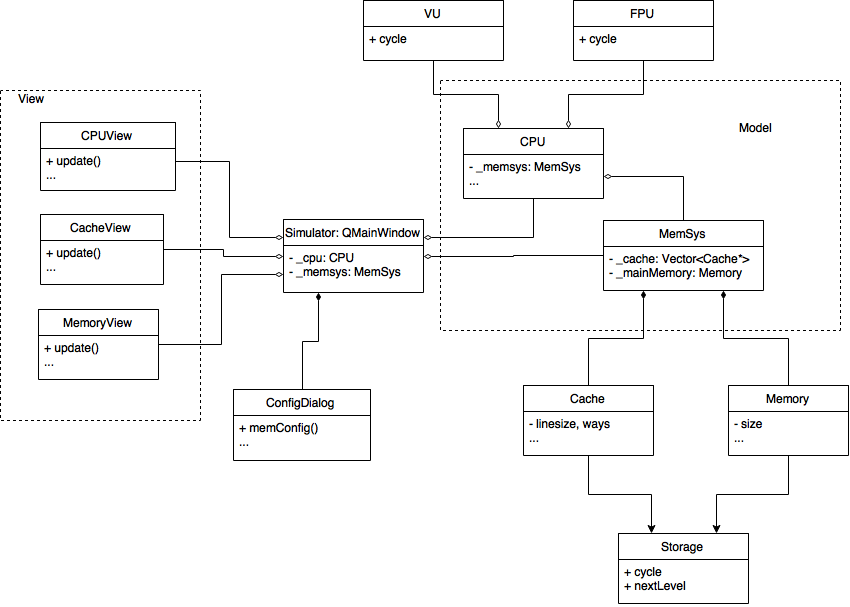
\includegraphics[width = 0.7\linewidth,keepaspectratio]{uml_simulator}
\caption{Overview of simulator architecture}
\label{fig:uml}
\end{figure*}

\subsection{Memory and cache system}
We use a hierarchical structure to build the memory-cache system. First, we define an abstract class called \texttt{Storage}. Both \texttt{Cache} and \texttt{Memory} inherits from this base class. The \texttt{Storage} class contains an integer field \texttt{cycle} defining the number of cycles it needs to execute an instruction and a pointer \texttt{nextLevel} that references to the next level of storage object, if any. It also supports 3 methods \texttt{load}, \texttt{store} and \texttt{dump}. The \texttt{load} method takes a 32-bit integer address, a pointer to the buffer for storing loaded values and the length of the memory blocks to be read as the arguments. It copies the content in the memory starting at the address into the buffer of the same size. The \texttt{store} method takes the same three arguments as the \texttt{load} method. Instead of loading the blocks into the buffer, it takes the content from the buffer and writes them into the blocks from the starting address. The \texttt{dump} method converts and concatenates the content in the storage into a string for debugging.  

\subsubsection{Memory}
The \texttt{Memory} class inherits from the \texttt{Storage} class, it implements the methods inherited from the \texttt{Storage} class straight forwardly. The data is stored in an byte array so it is byte addressable. The pointer to the next level is set to be a null pointer. 

\subsubsection{Cache}
An overview of the cache memory hierarchy is shown in Figure \ref{fig:cache_vs_memory}. The \texttt{Cache} class we implemented supports multiple-way associativity with write back/through and LRU/Random policies. The \texttt{Cache} class also inherits from the \texttt{Storage} class. It consists of multiple cache lines as the basic building block.

\begin{figure*}[!ht]
\centering
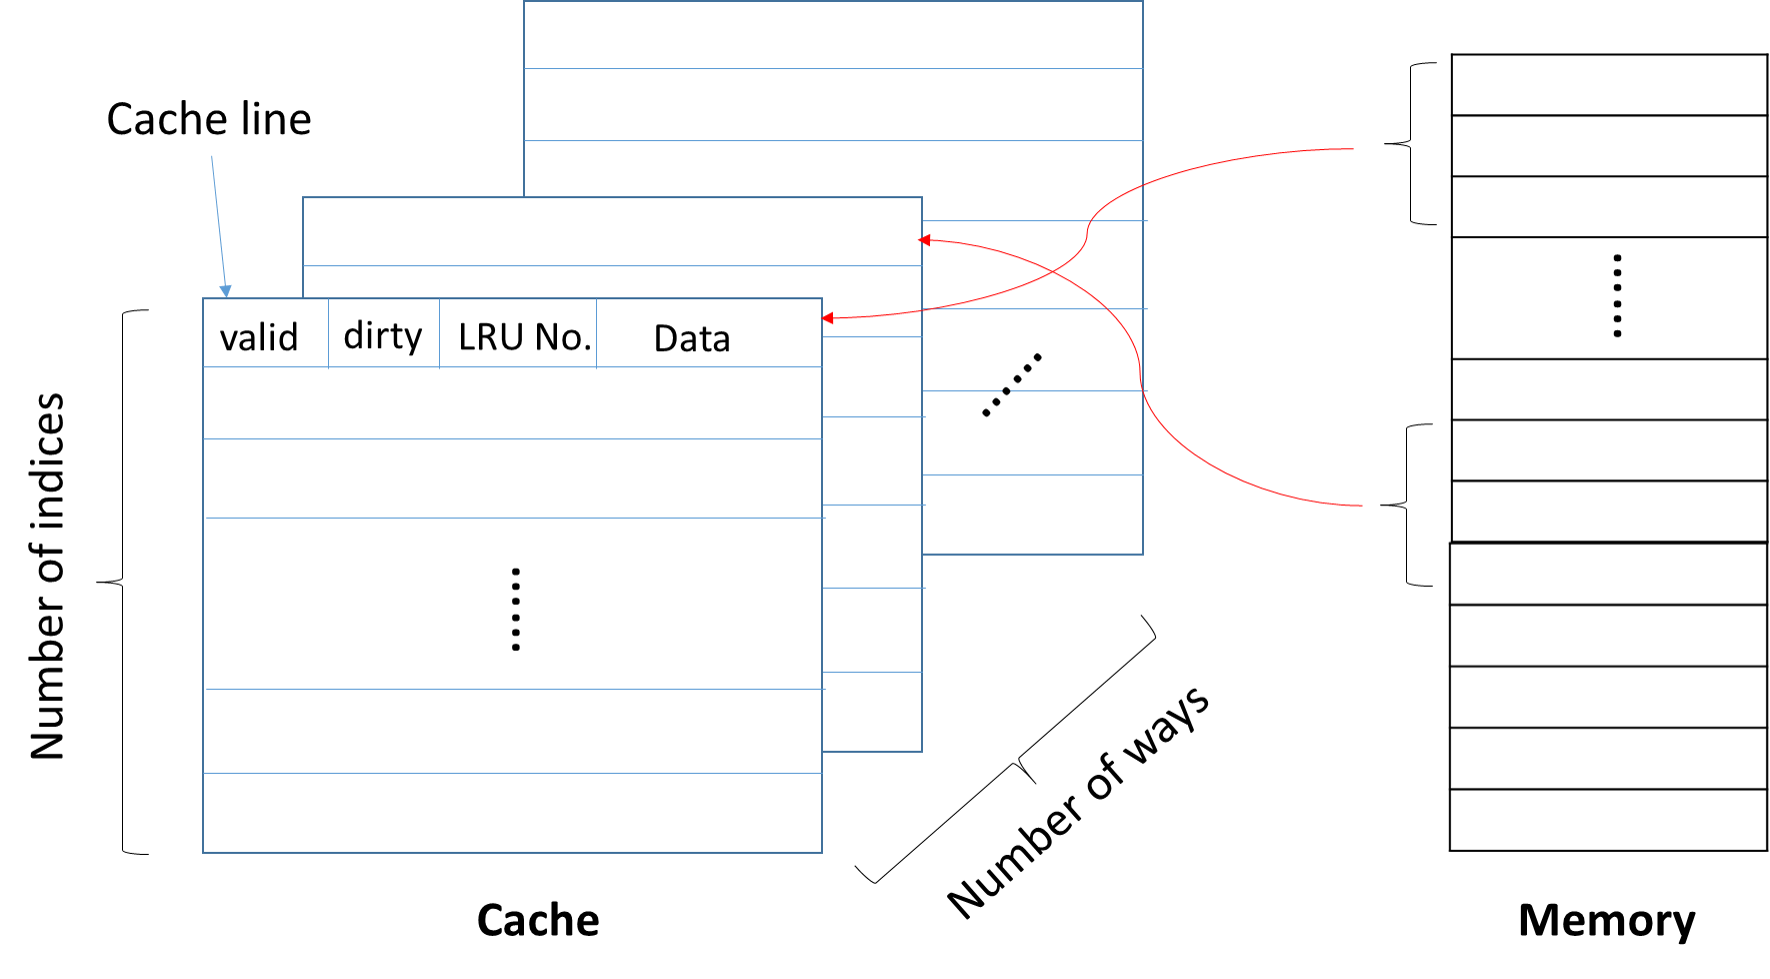
\includegraphics[width = 0.7\linewidth,keepaspectratio]{Cache_and_Memory.png}
\caption{Schematic of memory and cache implementation}
\label{fig:cache_vs_memory}
\end{figure*}

\paragraph{Cache line}
 The cache line is defined using the struct \texttt{Cacheline}. It has a boolean field called \texttt{valid} that indicates if this cache line is empty or not, a boolean field \texttt{dirty} that indicates if the content in the cache line is newer than that in the lower level storage. The \texttt{lru} field indicates its priority in the LRU replacing mechanism. It also contains a pointer \texttt{data} referencing to an array of bytes that served as the data blocks.

The cache consists of a two-dimensional array of \texttt{Cacheline}. The rows correspond to indices of memory blocks and the columns correspond to the ways associated to the same index. The total size of cache is the number of rows times the number of columns. The size of the cache, number of ways and number of index can be set at the initialization stage.

\paragraph{Cache functions}
The \texttt{inCache} method takes an address and returns the cache line position if the address exists in the cache or null if not. Since the memory address starts from 0, it calculates the block index as (address / cache line size) and tag value as (address $\%$ cache line size). The block index corresponds to the index in the cache array. Then it iterates all the ways of cache lines attached to that index to see if any tag matches the tag of this address. If there is any match, it returns the position of the cache line, otherwise null. 

The \texttt{evict} method takes a requested address and returns a clean cache line position corresponding to that address. It looks up in the cache line array and searches for any empty lines of that address, which means that the valid flag is false. If such line exists, it returns its position. If all lines are occupied, which means all valid flags are true, it evicts a line according to the replace policies. We have implemented two replace policies: (1) random eviction (2) LRU eviction. Under the former scenario, a random number between $[0, \mathrm{number\ of\ ways} - 1]$ is generated. If the dirty bit of this cache line is true, which means it contains newer value than the lower level of storage, it will be evicted to the lower level of storage. Then the cache line is emptied and the position of it is returned. The LRU is implemented as follows. Each cache line at a specific index is assigned an LRU number. When a line at this index is updated, all other lines that have lower LRU numbers are incremented by 1. Then the visited line's LRU number is set to 0. The higher number means less recently used. 

The \texttt{load} method allows us to read a block starting at a specific address in memory. It first checks if the address exists in the current cache level by calling the \texttt{inCache} method. If the returned position is null, there is a cache miss. It will call the the next level of storage's \texttt{load} method, which could be another cache or the memory. The data will be passed along the hierarchical call chain. The newly loaded data have to be written into the cache. An empty cache line is created by calling the \texttt{evict} method. If the returned position is not null, there is a cache hit. The data in the current cache line is loaded and passed up. 

The \texttt{store} method allows us to write an array of data blocks into a specific address in memory. First, it also checks if the cache line corresponding to the requested address exists in the cache by calling the \texttt{inCache} method. If yes, it reports a cache hit and copies the data blocks into the current level of cache. Two write policies are implemented: (1) write back (2) write through. In the former scenario, we just set the dirty flag of the cache line to be true, update the LRU numbers and done. In the latter scenario, we still need to call the \texttt{store} method in the next level of storage to pass the data down. If the address doesn't have a corresponding cache line in the cache, we have a cache miss. The \texttt{load} method is called to bring the data blocks from next level into the cache. Then it's treated as in the cache hit case. 
% multiple-way associative cache with write allocate, LRU 
 
\subsubsection{Memory system}
The \texttt{MemSys} acts as a mediator between the cache-memory hierarchy and CPU. Both \texttt{Memory} and \texttt{Cache} are encapsulated in it. The \texttt{MemSys} class exposes four methods \texttt{loadWord}, \texttt{loadByte}, \texttt{storeWord}, \texttt{storeByte} for CPU fetching instructions or issuing load/store instruciton. It also keeps a \texttt{countdown} integer for CPU clocking. Each time CPU issues an request, it calculates the required cycles to complete that request and only return the result after that cycle has passed. Internally, \texttt{MemSys} uses a string \texttt{request} keeping the current serving request, if a different request comes in (possible under the pipeline mode), it will not respond until it finishes its current serving request. That means this memory system has only one port and only allows a single access at a time. 

The \texttt{MemSys} is also responsible for communication between the \texttt{Simulator} class. Whenever the \texttt{Memory} or \texttt{Cache} changes its internal status, it will emit a notifying signal to the \texttt{Simulator}, and \texttt{Simulator} will in turn call the update methods in the corresponding view. \texttt{Simulator} can talk to the \texttt{MemSys} to change its configuration. When a user modifies the memory system configuration in the \texttt{ConfigDialog} class, the \texttt{Simulator} will notify \texttt{MemSys} through signaling and \texttt{MemSys} will initialize a new setting of cache-memory hierarchy by calling the \texttt{init} method.

\texttt{MemSys} provides one layer of indirection. It hides the implementation of the cache and memory and makes the interfaces between other classes easier to maintain. 

\subsection{CPU}
The \texttt{CPU} class is where most of the simulation happens. This class keeps a \texttt{clk} field for clock cycle, a \texttt{pc} field for the program counter, and also the register files and pipeline states. It maintains a pointer to the \texttt{MemSys} for memory access and pointers to a \texttt{FPU} and a \texttt{VU} for special instructions. Besides, it can communicate with \texttt{Simulator} to notify the update of CPU status and get the commands from the user interface.
\begin{figure}[!ht]
\centering
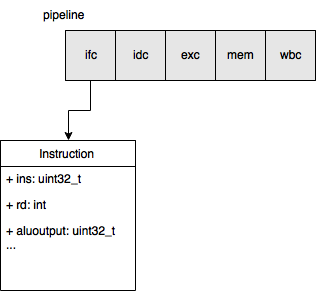
\includegraphics[width = 0.7\linewidth,keepaspectratio]{pipeline}
\caption{Pipeline structure}
\label{fig:pip}
\end{figure}

\begin{figure*}[!ht]
\centering
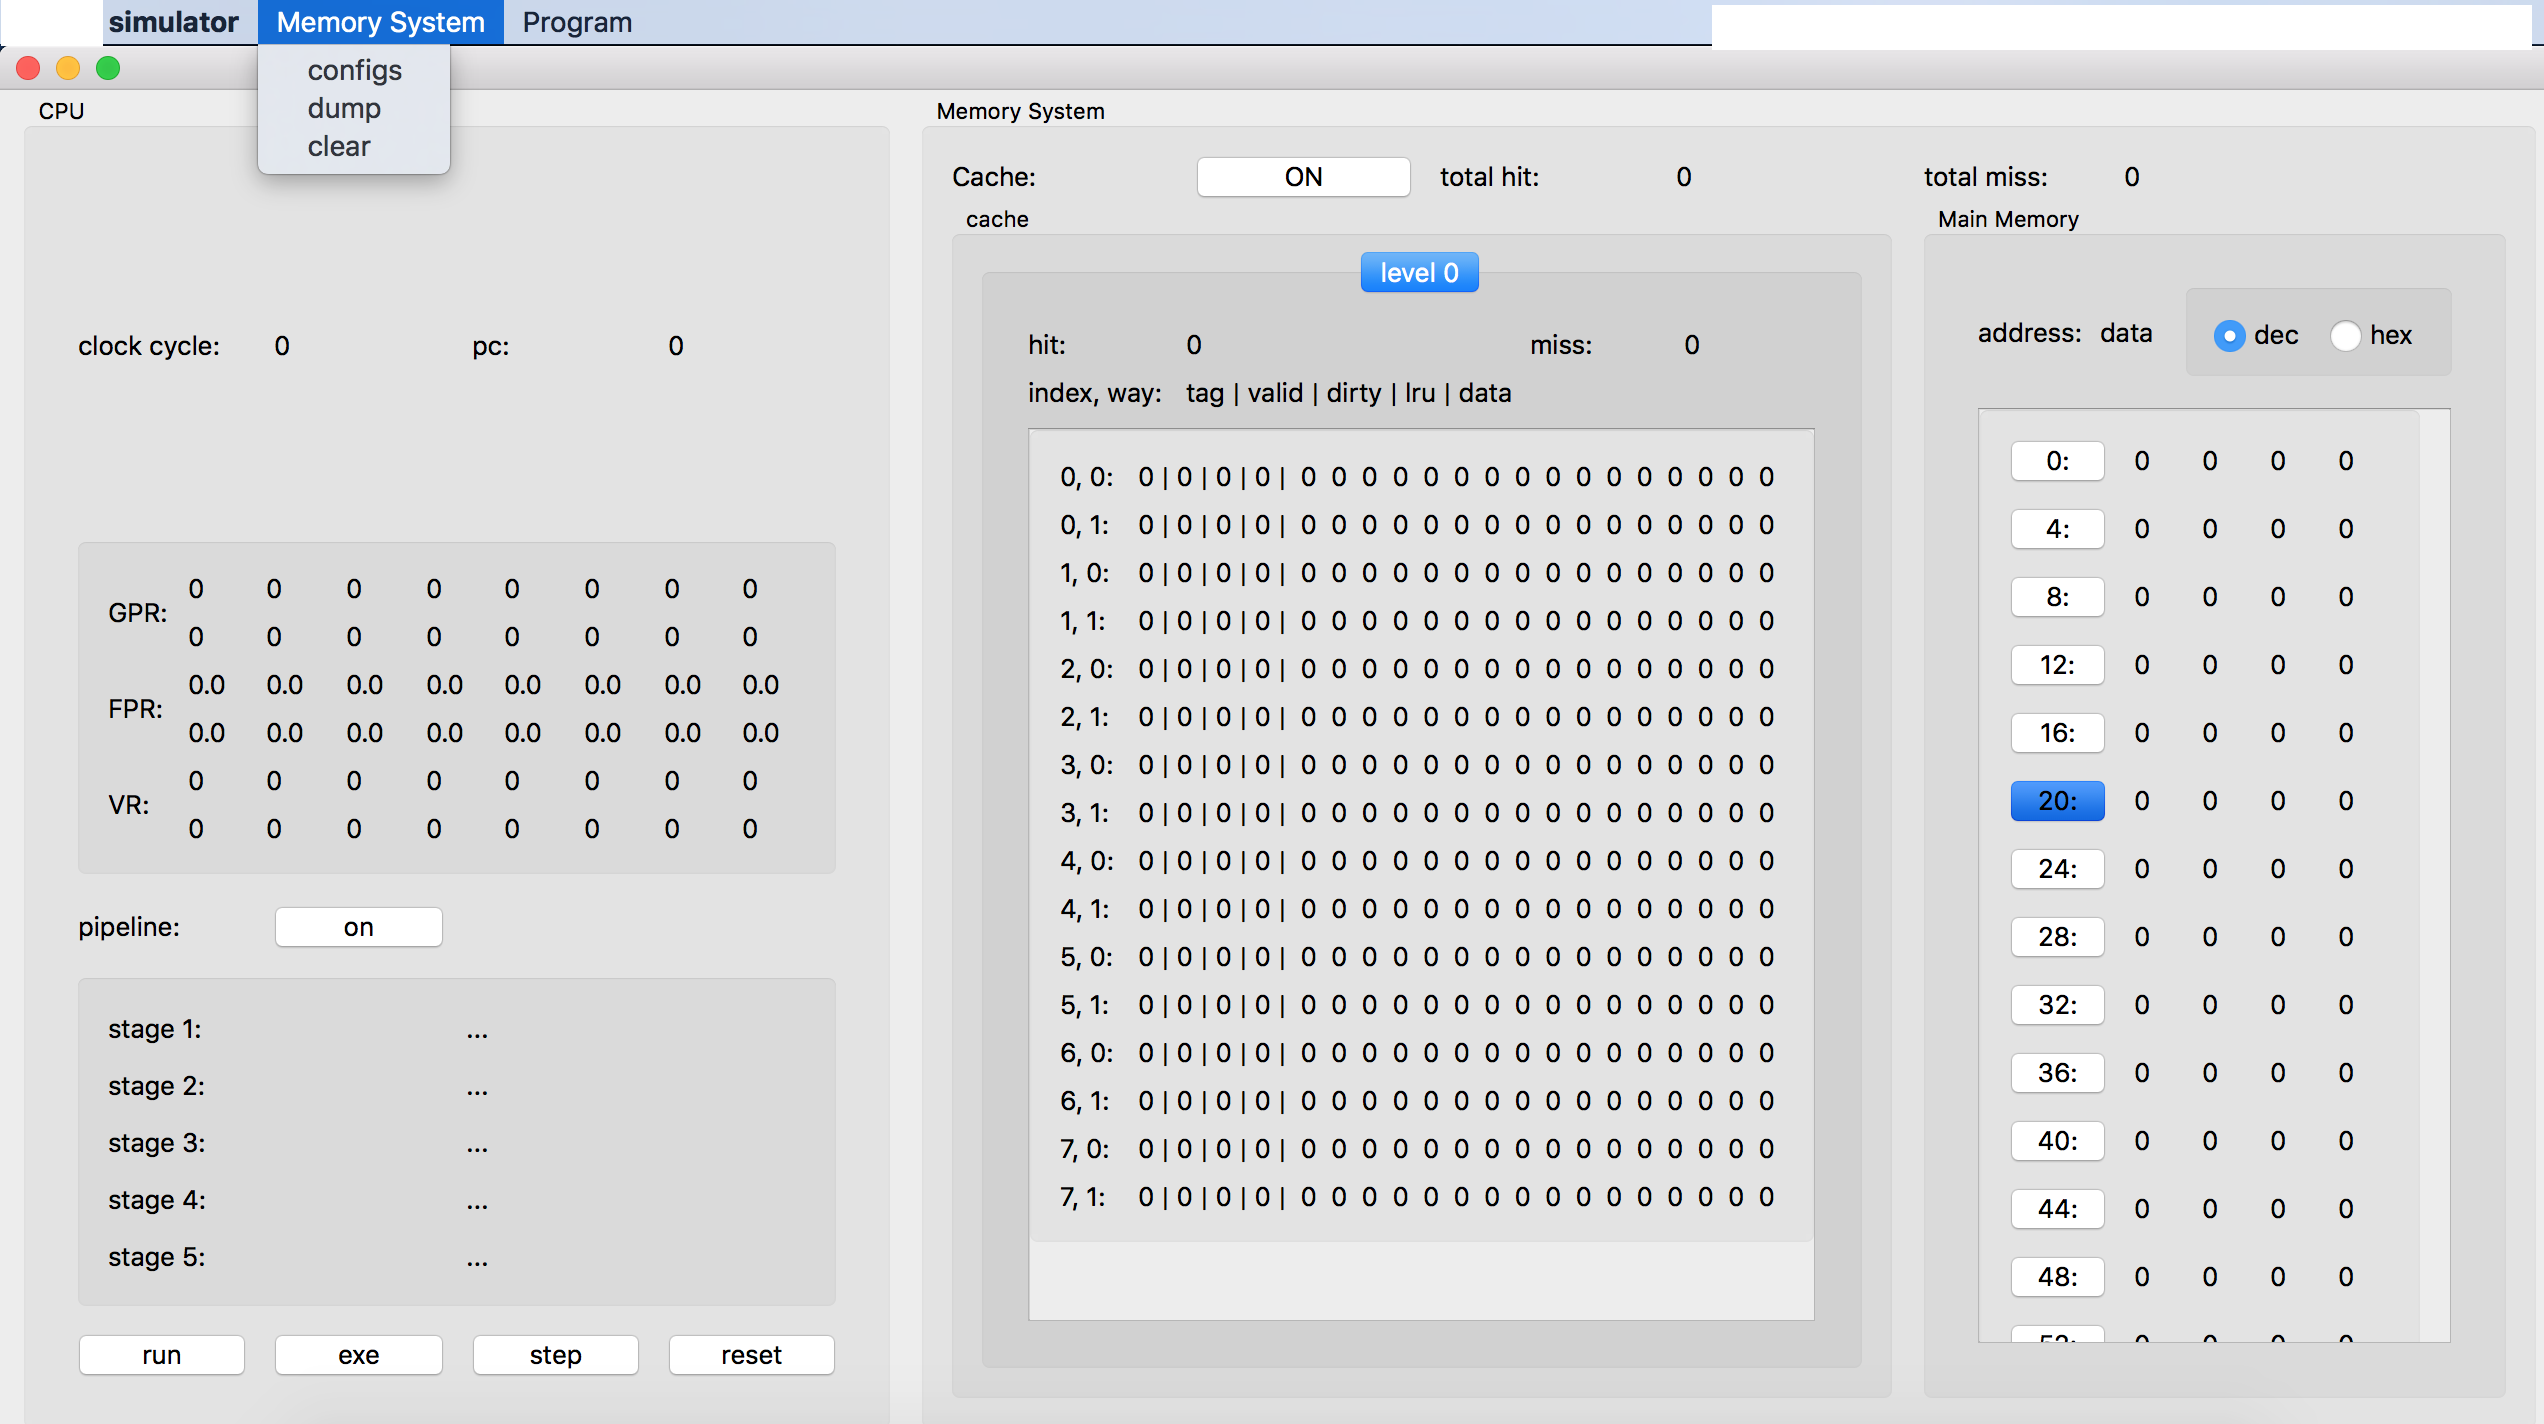
\includegraphics[width = 0.7\linewidth,keepaspectratio]{gui}
\caption{GUI screenshot}
\label{fig:gui}
\end{figure*}

\subsubsection{Pipeline}
The \texttt{CPU} class uses a standard 5-stage MIPS pipeline. Every instruction can be completed in 5 cycles: instruction fetch cycle (ifc), instruction decode cycle (idc), execution cycle (exc), memory access cycle (mem) and write-back cycle (wbc). There are five methods \texttt{ifc}, \texttt{idc}, \texttt{exc}, \texttt{mem} and \texttt{wbc} implementing these cycles. The pipeline \texttt{pipe} is implemented as a array of length 5. Each position in the array corresponds to a execution stage (see Figure \ref{fig:pip}). Elements in the array are the structure \texttt{Instruction}. \texttt{Instruction} keeps information about the instruction being executed. It resembles the registers between pipeline stages in hardware. Some key fields are \texttt{opcode} for keeping instruction code, \texttt{rd1}, \texttt{rd2}, \texttt{rd3}, \texttt{imm} for storing operands, \texttt{stage} for indicating execution stage and \texttt{aluoutput}, \texttt{fpuoutput}, \texttt{vuoutput}, \texttt{lmd} for keeping execution cycle result. The execution of the instruction is simulated by passing the structure through the \texttt{pipe} array and filling its fields in different stages. 

\paragraph{ifc}
Fetch instructions from \texttt{MemSys} by calling \texttt{loadWord} method and create a \texttt{Instruction} instance. If in a pipelined execution mode, examine the instruction at \texttt{mem} stage to see if it is a branch. If it is a branch and it is taken, change the \texttt{pc} accordingly. Otherwise increase the \texttt{pc} by 4. If the next stage in \texttt{pipe} is empty, change its \texttt{stage} to 1 and pass the structure to the next stage.  

\paragraph{idc}
Decode the instruction. First extract the 7 bits to get the instruction opcode, and then decode the rest operands according to the format (Table \ref{tab:if}). After decoding, load operands from register files. If under the pipelining mode, we need to resolve potential data hazards. In the 5-stage pipeline setting, we only need consider read after write (RAW) hazard since the write back cycle is at the last stage and only one instruction can write at a time. Examine every instruction in the pipeline after idc stage and see if its destination register is one of the operands we need to read. If the instruction has finished its execution, we can forward the result in \texttt{aluoutput} (or \texttt{fpuoutput}, \texttt{vuoutput}, \texttt{lmd}) to the operand we need. Otherwise, we need to stall the pipeline, and wait for the operand to be ready. When the operands are ready, we can pass the instruction to the next stage.

\paragraph{exc}
Execute the instruction according to its opcode. If it only needs integer computation, we can finished the execution within the \texttt{CPU} class, otherwise, we need to forward the instruction to \texttt{FPU} or \texttt{VU} for special handling. In \texttt{CPU}, we can do data transfer, arithmetic and logical, control and cache instruction execution. If it is data transfer, we compute the memory address and store it in \texttt{aluoutput}. If it is arithmetic and logical, we save the computation result in \texttt{aluoutput}. And if it is control, we calculate the new \texttt{pc} address and put it in \texttt{aluoutput}. If it is floating point, we forward the instruction to \texttt{FPU} and wait for the result to store in \texttt{fpuoutput}. Similarly, SIMD instruction will be forwarded to \texttt{VU} and result saved in \texttt{vuoutput}. After computation, the instruction is passed to the mem stage.

\paragraph{mem}
This stage is only for data transfer instructions. If it is a load instruction, we load memory use the address stored in \texttt{aluoutput} and put it into \texttt{lmd}. If it is a store instruction, we store the value in operand to the address in \texttt{aluoutput}. Other type of instructions can directly pass this stage if the next stage is empty.

\paragraph{wbc}
Write \texttt{aluoutput} (or \texttt{fpuoutput}, \texttt{vuoutput}, \texttt{lmd}) to destination registers and destroy the \texttt{Instruction} structure.

The \texttt{step} method calls each stage function in reverse order (from \texttt{wbc} to \texttt{ifc}) and increase the \texttt{clk} by 1 afterwards. This completes one step of simulation. To simulating the whole program, we can call \texttt{step} until there are no more instructions. 


\subsubsection{FPU}
\texttt{FPU} handles floating point operations. It can simulate multi-cycle floating point calculations. Internally, it has a \texttt{cycle} and \texttt{countdown} field. Like \texttt{MemSys}, it will only respond requests from \texttt{CPU} after certain number of cycles. Since it is separated from \texttt{CPU}, for future extension, the pipeline can support multi-issue easily. 

\subsubsection{VU}
\texttt{VU} deals with vector operations. It also support multi-cycle calculation. Internally, vectors are saved as an array of bytes and computations are element wise. The separation of \texttt{VU} is also for future implementation of multi-issue.

\subsection{User interface and use guide}
The graphical interface is implemented in QT. A screenshot of the GUI is shown in Figure \ref{fig:gui}. The main window is the \texttt{Simulator} class. It can be roughly divided into three parts. 

The left panel is for displaying CPU status which is implemented by \texttt{CPUView} class. Clock cycle, program counter, register files and pipeline can be seen here. There are also several buttons controlling the simulation. Pipeline \texttt{on}/\texttt{off} button can turn on/off the pipeline. \texttt{step} can simulate one clock cycle. \texttt{run} button executes the program at the speed of 100 millisecond one cycle. In this mode, you can see the changes in CPU or memory system easily. You can also stop the simulation whenever you want. \texttt{exe} button runs the program at full speed. Usually you can only see the final status of the program. \texttt{reset} button can clear the pipeline and register files and set the clock and pc to 0. 

The middle panel is for visualizing cache. It has tabs for switching between different level of caches and on the top, there is an \texttt{on}/\texttt{off} button for turning on/off cache. When the cache is turned off, the tab panel will become invisible. This part is implemented by \texttt{CacheView}. 

Finally, the right part is \texttt{MemoryView} where you can observe memory data and also change the display format. At the scroll area, you can press the address button and add or remove a breakpoint to the program. If the button is pressed down (turn blue), it means it is a breakpoint. 

You can change system configurations using the \texttt{configs} menu. After clicking the menu, a dialog (see Figure \ref{fig:conf}) will show up. New cache and memory configurations can be set here. This dialog is a class of \texttt{ConfigDialog} and is a component of \texttt{Simulator}. The \texttt{Memory System} also provides options to dump the memory data into a file or clear the memory. The \texttt{Program} provides a way to load program direct into memory. 
\begin{figure}[!ht]
\centering
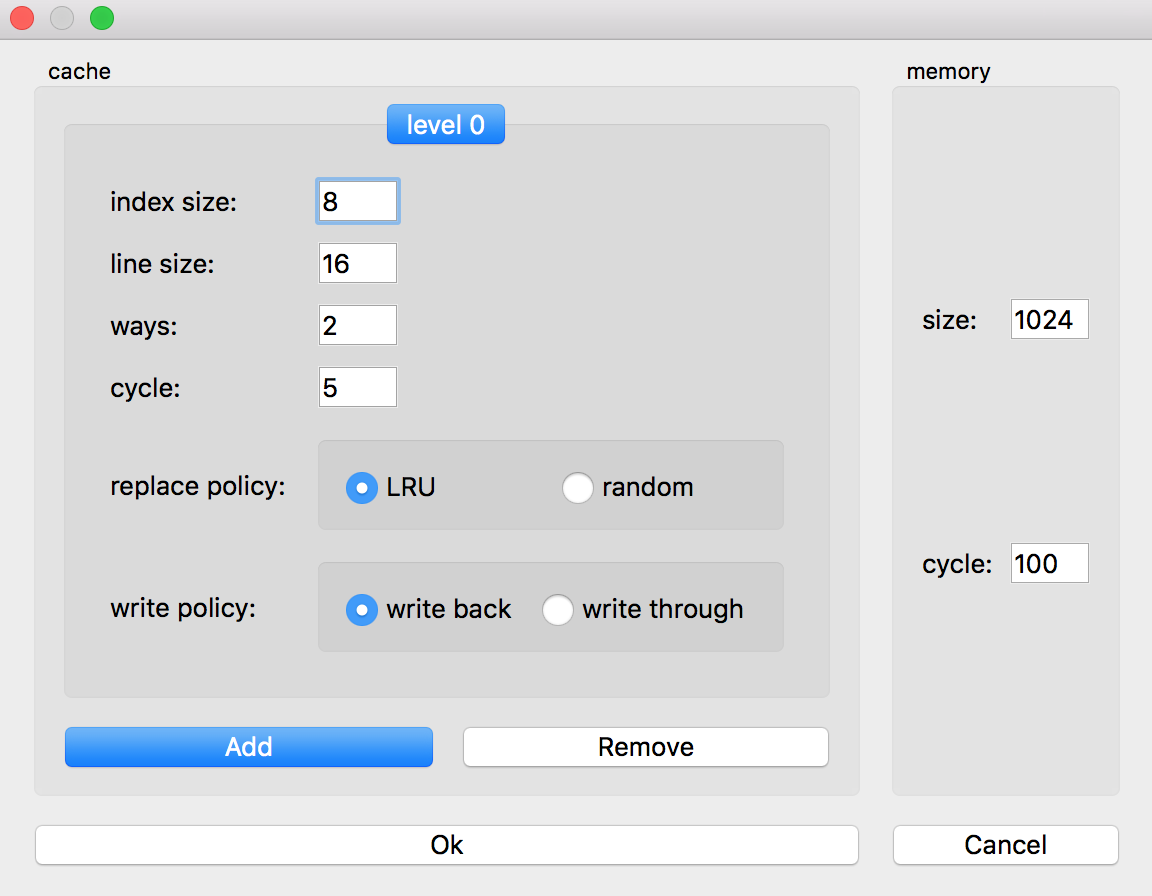
\includegraphics[width = 0.8\linewidth,keepaspectratio]{config}
\caption{Configuration Dialog}
\label{fig:conf}
\end{figure}

\subsection{Assembler }
The assembler takes the instructions in assembly language and encodes them into 32-bit integers. The assembler executes in two passes. In the first pass, it strips all the comments that starts with $\#$ symbol and stores all labels into a label map, which use the line number as the value. In the second pass, it replaces the labels in other clauses with the relative line numbers and encodes the instructions according to a preloaded map of opcodes. The result is written in binary format into a file. 


\subsection{Testing}
We tested our simulator mainly through GUI. To test the memory system, we wrote a program generating sequential or random memory accessing instructions. Then we use a small drive program to read in these instructions and directly call the interface provided by \texttt{MemSys}. For sequence access, we precomputed the final cache-memory state manually and compare with the result produced by simulator. In this way, we found a bug in cache line eviction. For random access, since the result is hard to compute by hand, we only see if a large amount of random accesses will break the program. The simulator has passed this stress test.

To test the assembler, we simply wrote a disassembler and to see the results converted from each side match. We also manually encoded the benchmark program exchange sort to see if the assembler works.
 
To test the pipeline, we designed some small programs with data dependencies and branch hazards. We run the simulator step by step to see if it can handle the hazard correctly. In this way, we found some bug in implementing branch instructions.

\section{Performance evaluation}
\subsection{Benchmark}
We designed the following benchmark programs: (1) Exchange sort (2) Matrix multiplication (3) Matrix multiplication with SIMD for performance evaluation. 

The exchange sort uses the bubble sort algorithm (Algorithm 1). Core part is two level of \texttt{for} loop. We implement the \texttt{if} condition with \texttt{bgez} instruction and the \texttt{for} loop condition with \texttt{beq} instruction.

\begin{algorithm}[h]
\SetAlgoLined
 integer array A; l = length of A\;
 \For{ i from 0 to l - 2}{
	\For{ j from i + 1 to l - 1} {
    	\eIf{A[i] > A[j]}{
        	swap A[i] and A[j]\;
        }{continue;}
    }
 }
\caption{Exchange sort}
\end{algorithm}

Matrix multiplication uses a three level of \texttt{for} loop (Algorithm 2). The \texttt{for} loops are also implemented in \texttt{beq} instruction. In the experiment, we will multiply a 4 by 8 matrix with a 8 by 4 matrix.

\begin{algorithm}[h]
\SetAlgoLined
 left matrix L ($4 \times 8$), right matrix R ($8 \times 4$)\;
 a = number of rows in L, b = number of columns in L\;  
 c = number of columns in R\;
 Create result matrix res of size a*c, initialized with 0s\;
 \For{ i from 0 to a - 1}{
	\For{ j from 0 to c - 1}{
    	\For{ k from 0 to b - 1}{
        	res[i][j] += L[i][k]*R[k][j]\;
        }
    }
 }
 return res\;
 \caption{Matrix multiplication}
\end{algorithm}

Matrix multiplication with SIMD uses the same size matrix as above. Since the architecture supports 8-byte vector multiplication, we can preload rows and columns of the matrix into the vector and do the multiplication in one step. The result matrix can be calculated using the formula in Algorithm 3. From experiment results, we can see SIMD saves CPU cycles. 

\begin{algorithm}[h]
\SetAlgoLined
 left matrix L, right matrix R\;
 Flatten L into a vector v1 of size 8 by rows\;
 Flatten R into a vector v2 of size 8 by columns\;
 Create result matrix res of size 4, initialized with 0s\; 
 Create vector v3 with size 8\;
  \For{ i from 0 to 3}{
	\For{ j from 0 to 3}{
	v1 =  L[i][], v2 = R[][j]\;	
	v3 = v1 * v2\;
	res[i][j]  =  sum(v3)\;
	
    }
 }
 return res\;
 \caption{Matrix multiplication with SIMD}
\end{algorithm}

\subsection{Experiment result}
We tested our three benchmarks under 10 cache configurations and with or without pipeline being turned on and measured their performance in terms of total CPU cycles being used. Configuration details can be found in Table \ref{tab:conf}. Memory cycle is assumed to be 100. L1 cache is 5 cycle and L2 cache is 20 cycle. Simulation results are shown in Table \ref{tab:res}. 
\begin{table}[!ht]
\caption{Cache Configurations}
\label{tab:conf}
\centering
\begin{tabular}{|c|c|c|c|c|c|}
\hline
 & level & index size & ways & line size & policy \\ \hline
 1 & 1& 4 & 1& 8& -\\
\hline
 2 & 1& 4 & 1& 16 & -\\
\hline
 3 & 1& 4 & 4& 8& LRU\\
\hline
 4 & 1& 4 & 4& 8& Rand\\
\hline
 5 & 1& 4 & 4& 16& LRU\\
\hline
 6 & 1& 4 & 4& 32& LRU\\
\hline
 7 & 2 & 4,16 & 1,2& 8,16& LRU\\
\hline
 8 & 2 & 4,16 & 2,2& 8,16& LRU\\
\hline
 9 & 2 & 4,16 & 1,2& 16,16& LRU\\
\hline
 10 & 2 & 4,16 & 2,2& 16,32& LRU\\
\hline
\end{tabular}
\end{table}

\begin{table*}[!ht]
\caption{Evaluation result}
\label{tab:res}
\centering
\begin{tabular}{|c|c|c|c|}
\hline
 Setting & Exchange Sort & Matrix Multiplication  & Matrix Multiplication with SIMD\\

 & & ($4\times8 * 8 \times 4$) & ($4\times8 * 8 \times 4$) \\ \hline
baseline & 72451 & 223956 & 48580 \\
\hline
cache configure 1& 55696 & 135996 & 35860 \\
\hline
cache configure 2 & 28796 & 75696 & 23560\\
\hline
cache configure 3 & 7496& 41596& 14460\\
\hline
cache configure 4 & 30596& 123896& 32560\\
\hline
cache configure 5& 6296& 20096 & 7260 \\
\hline
cache configure 6 & 5796 & 17796 & 5260 \\
\hline
cache configure 7 & 16416 & 43676 & 13360\\
\hline
cache configure 8 & 11336 & 33456 & 11220\\
\hline
cache configure 9 & 11036 & 31616 & 10900 \\
\hline
cache configure 10 & 6036 & 21236 & 7160 \\
\hline
pipeline &70847 & 218620 & 47500 \\
\hline
pipeline + cache configure 1 & 47592 & 135960 & 34680\\
\hline 
pipeline + cache configure 2 & 18492 & 73960 & 23580\\
\hline
pipeline + cache configure 3 & 5792 & 34460 & 12380\\
\hline
pipeline + cache configure 4 & 28092 & 123560 & 30680\\
\hline
pipeline + cache configure 5 & 4692 & 14660 & 6080\\
\hline 
pipeline + cache configure 6 & \textbf{4192}& \textbf{12560} & \textbf{4080}\\
\hline
pipeline + cache configure 7 & 13512& 39300& 12160\\
\hline
pipeline + cache configure 8 & 8452& 28900& 10140\\
\hline
pipeline + cache configure 9 & 7692& 26900& 9940\\
\hline
pipeline + cache configure 10 & 4432& 15420& 5800\\
\hline
\end{tabular}
\end{table*}

From the table, we can see that overall cache configuration 6 with pipeline achieves the best performance and SIMD is better than using loop for matrix multiplication. Further comparing different results, we can find the following interesting conclusions. (1) pipeline itself does not provide much improvement. Without cache, pipeline can only provide about 2\% cycles reduction. But with cache, it can provide over 10\% boost. (2) pipeline may lower the performance if the cache configuration is not right. We observed that cycle numbers increased for cache configuration 2  running the matrix multiplication program. The increase of cycle numbers may be due to that two instructions in the pipeline need to access the same cache line but with different memory address. This only happens when cache is direct-mapped. (3) cache makes a huge difference for performance. With a bigger and more associative cache, performance can boost over 500\%, (for example comparing configuration 1 and 3). (4) finding the right cache configuration is difficult. Generally more associative and bigger cache line size will help. Adding L2 cache does not help much compared with expanding the number capacity. (5) LRU is much better than random when the number of ways is large. Comparing configuration 3 and 4, LRU has a huge advantage. (6) program instruction types also play a big role. Programs with more branching and memory access have more potential to be optimized. 

\section{Summary}
We gained lots of experience in designing and implementing a standalone system from the scratch. A couple of lessons have been learned:

For the experiment result, we learned that pipeline has to work with cache to provide better performance and memory is usually the bottle neck of the program. A good cache will help boosting the performance a lot. 

During the implementation of the simulator, we learned that having a good design at first is extremely important. For example, before adapting the signal and slot model and using simulator as a mediator, we used the callback function and let classes directly talk to each other. After many functions were added, the interaction between them became too complicated to maintain. But usually it is hard to have a good design at the beginning, so redesign early is also very helpful. 

We also learned testing is hard and manually test is not practical and efficient. The memory is relatively easy to test because we can treat it like a black box. But cache and CPU is hard to use blackbox test. Manually writing test is time-consuming and makes it less efficient in debugging.

\begin{table*}[p]
\caption{Instruction List}
\label{tab:il}
\centering
\begin{tabular}{|c|l|c|l|p{8cm}|}
\hline
Type & Instruction & Encoding & Format & Description \\
 \hline
\multirow{6}{*}{Data Transfer} & lb & 0010000 & lb \$1,\$2,im & load mem[\$1+im] and sign extended into gpr[\$2] \\ \cline{2-5}
 & lbu & 0010001 & lbu \$1,\$2,im & load mem[\$1+im] into gpr[\$2] \\ \cline{2-5}
 & sb & 0011000 & sb \$1,\$2,im & store lower 8 bits of gpr[\$2] into mem[\$1+im] \\ \cline{2-5}
 & lw & 0010010 & lw \$1,\$2,im & load mem[\$1+im ... \$1+im+3] into gpr[\$2]\\ \cline{2-5}
 & sw & 0011001 & sw \$1,\$2,im & store gpr[\$2] into mem[\$1+im ... \$1+im+3]\\ \cline{2-5}
 & lsp & 0010100 & lsp \$1,\$2,im & load mem[\$1+im ... \$1+im+3] into fpr[\$2] \\ \hline
\multirow{23}{*}{Arithmetic \& Logical} & add & 1000000 & add \$1,\$2,\$3 & gpr[\$3] = gpr[\$1] + gpr[\$2] \\ \cline{2-5}
 & sub & 1000001 & sub \$1,\$2,\$3& gpr[\$3] = gpr[\$1] - gpr[\$2] \\ \cline{2-5}  
 & addi & 1010011 & addi \$1,\$2,im & gpr[\$2] = gpr[\$1] + im \\ \cline{2-5}
 & subi & 1010100 & subi \$1,\$2,im &  gpr[\$2] = gpr[\$1] - im \\ \cline{2-5}
 & mul & 1000010 & mul \$1,\$2,\$3 & gpr[\$3] = lower 32 bits of (gpr[\$1]*gpr[\$2] as signed value) \\ \cline{2-5}
 & muh & 1000011 & muh \$1,\$2,\$3 & gpr[\$3] = higher 32 bits of (gpr[\$1]*gpr[\$2] as signed value) \\ \cline{2-5}
 & mulu & 1000100 & mulu \$1,\$2,\$3 & gpr[\$3] = lower 32 bits of (gpr[\$1]*gpr[\$2] as unsigned value) \\ \cline{2-5}  
 & muhu & 1000101 & muhu \$1,\$2,\$3 &  gpr[\$3] = higher 32 bits of (gpr[\$1]*gpr[\$2] as unsigned value) \\ \cline{2-5}
 & div & 1000110 & div \$1,\$2,\$3 & gpr[\$3] = gpr[\$1] / gpr[\$2] as signed value \\ \cline{2-5}
 & divu & 1000111 & divu \$1,\$2,\$3 & gpr[\$3] = gpr[\$1] / gpr[\$2] as unsigned value \\ \cline{2-5}
 & modu & 1001000 & modu \$1,\$2,\$3 & gpr[\$3] = gpr[\$1] \% gpr[\$2] as unsigned value \\ \cline{2-5}
 & and & 1001001 & and \$1,\$2,\$3 & gpr[\$3] = gpr[\$1] \& gpr[\$2] \\ \cline{2-5}  
 & or & 1001010 & or \$1,\$2,\$3 & gpr[\$3] = gpr[\$1] | gpr[\$2] \\ \cline{2-5}
 & not & 1001011 & not \$1,\$0,\$3 & gpr[\$3] = $\sim$ gpr[\$1]  (\$0 is not relevant but required) \\ \cline{2-5}
 & xor & 1001100 & xor \$1,\$2,\$3 & gpr[\$3] = gpr[\$1] $\wedge$ gpr[\$2] \\ \cline{2-5}
 & rr & 1001101 & rr \$1,\$2,\$3 &  gpr[\$1] rotate right \$2 bits and store in gpr[\$3] \\ \cline{2-5}
 & srl & 1001110 & srl \$1,\$2,\$3 & gpr[\$1] logical shift right \$2 bits and store in gpr[\$3]  \\ \cline{2-5}  
 & sra & 1001111 & sra \$1,\$2,\$3 & gpr[\$1] arithmetic shift right \$2 bits and store in gpr[\$3]  \\ \cline{2-5}
 & sl & 1010000 & sl \$1,\$2,\$3 & gpr[\$1] shift left \$2 bits and store in gpr[\$3]  \\ \cline{2-5}
 & slt & 1010001 & slt \$1,\$2,\$3 & gpr[\$3] = (gpr[\$1] < gpr[\$2]) as signed value \\ \cline{2-5}
 & sltu & 1010010 & sltu \$1,\$2,\$3 &  gpr[\$3] = (gpr[\$1] < gpr[\$2] ) as unsigned value \\ \cline{2-5}
 & slti &1010101 & slti \$1,\$2,im & gpr[\$2] = (gpr[\$1] < im) as signed value \\ \cline{2-5}
 & sltiu & 1010110 & sltiu \$1,\$2,im &  gpr[\$2] = (gpr[\$1] < im) as unsigned value\\ \hline
\multirow{9}{*}{Control} & j & 0000001 & j offset & jump to offset (\$pc = offset) \\ \cline{2-5}
 & jal & 0000010 & jal offset & jump to offset and put current \$pc to gpr[15] \\ \cline{2-5}  
 & beq & 0000011 & beq \$1,\$2,offset & branch an offset (\$pc = \$pc +offset) if gpr[\$1] == gpr[\$2] \\ \cline{2-5}
 & bneq & 0000100 & bneq \$1,\$2,offset & branch an offset (\$pc = \$pc +offset) if gpr[\$1] != gpr[\$2] \\ \cline{2-5}
 & bgez & 0000101 & bgez \$1,offset & branch an offset (\$pc = \$pc +offset) if gpr[\$1] >= 0 \\ \cline{2-5}
 & bgtz & 0000110 & bgtz \$1,offset & branch an offset (\$pc = \$pc +offset) if gpr[\$1] > 0 \\ \cline{2-5}
 & blez & 0000111 & blez \$1,offset &  branch an offset (\$pc = \$pc +offset) if gpr[\$1] <= 0 \\ \cline{2-5}  
 & bltz & 0001000 & bltz \$1,offset & branch an offset (\$pc = \$pc +offset) if gpr[\$1] < 0 \\ \cline{2-5}
 & break & 0000000 & break & break \\ \hline
 \multirow{7}{*}{Floating Point} & addsp & 0100000 & addsp \$1,\$2,\$3 & fpr[\$3] = fpr[\$1] + fpr[\$2] \\ \cline{2-5}
 & subsp & 0100001 & subsp \$1,\$2,\$3 & fpr[\$3] = fpr[\$1] - fpr[\$2] \\ \cline{2-5}  
 & mulsp & 0100010 & mulsp \$1,\$2,\$3 & fpr[\$3] = fpr[\$1] * fpr[\$2] \\ \cline{2-5}
 & divsp & 0100011 & divsp \$1,\$2,\$3 & fpr[\$3] = fpr[\$1] / fpr[\$2] \\ \cline{2-5}
 & sltsp & 0100100 & sltsp \$1,\$2,\$3 & fpr[\$3] = (fpr[\$1] < fpr[\$2])\\ \cline{2-5}
 & witf & 0100101 & witf \$1,\$2 & convert integer gpr[\$1] to floating point and store in fpr[\$2] \\ \cline{2-5}
 & wfti & 0100110 & wfti \$1,\$2 & convert floating point fpr[\$1] to integer and store in gpr[\$2]\\ \hline
 Cache & pref & 0110000 & pref \$1,\$0,im & load mem[\$1+im ... \$1+im+3] into cache (\$0 is not relevant but required) \\ \hline
 \multirow{15}{*}{SIMD} & move & 1101010 & move \$1,\$2 & vr[\$2] = vr[\$1] \\ \cline{2-5}
 & sum & 1101011 & sum \$1,\$2 & compute sum of bytes in vr[\$1] and store to gpr[\$2] \\ \cline{2-5}  
 & copy & 1101100 & copy \$1,\$2,n & copy n-th byte in vr[\$1] to gpr[\$2] as unsigned value\\ \cline{2-5}
 & insertb & 1101101 & insertb \$1,\$2,n & store lower 8 bits of gpr[\$1] to the n-th byte in vr[\$2] \\ \cline{2-5}
 & fillb & 1101110 & fiilb \$1,\$2 & fill lower 8 bits of gpr[\$1] to all bytes in vr[\$2] \\ \cline{2-5}
 & vaddb & 1100000 & vaddb \$1,\$2,\$3 & vr[\$1] = vr[\$2] + vr[\$3] \\ \cline{2-5}
 & vsubb & 1100001 & vsubb \$1,\$2,\$3 & vr[\$1] = vr[\$2] - vr[\$3]  \\ \cline{2-5}  
 & vmulb & 1100010 & vmulb \$1,\$2,\$3 & vr[\$1] = vr[\$2] * vr[\$3]  \\ \cline{2-5}
 & vdivb & 1100011 & vdivb \$1,\$2,\$3 & vr[\$1] = vr[\$2] / vr[\$3]  \\ \cline{2-5}
 & vmodb & 1100100 & vmodbb \$1,\$2,\$3 & vr[\$1] = vr[\$2] \% vr[\$3] \\ \cline{2-5}
 & ceqb & 1100101 & ceqb \$1,\$2,\$3 & vr[\$3] = (vr[\$1] == vr[\$2]) (element wise)\\ \cline{2-5}  
 & cleb & 1100110 & cleb \$1,\$2,\$3&vr[\$3] = (vr[\$1] <= vr[\$2]) (element wise, signed value)  \\ \cline{2-5}
 & cleub & 110111 & cleub \$1,\$2,\$3 & vr[\$3] = (vr[\$1] <= vr[\$2]) (element wise, unsigned value) \\ \cline{2-5}
 & cltb & 1101000 & cltb \$1,\$2,\$3 & vr[\$3] = (vr[\$1] < vr[\$2]) (element wise, signed value) \\ \cline{2-5}
 & cltub & 1101001 & cltub \$1,\$2,\$3 &vr[\$3] = (vr[\$1] < vr[\$2]) (element wise, unsigned value) \\ \hline
\end{tabular}
\end{table*}

\end{document}